\section{Plattform Hadoop"=Benchmark}
\label{sec:hadoopBenchmark}

\citeauthor{Zhang2016} haben im Rahmen ihrer gesamten Forschungsarbeit an der Selfbalancing"=Komponente darüber hinaus auch die Open"=Source"=Plattform Hadoop"=Benchmark\footnote{\url{https://github.com/Spirals-Team/hadoop-benchmark/}} entwickelt.
Sie dient zur einfachen und schnellen Ausführung eines Hadoop"=Clusters und wurde speziell zum Einsatz in der Forschung erstellt.
Dadurch kann sie auch mit geringem Aufwand an eigene Bedürfnisse angepasst werden.

Zur Ausführung des Clusters werden die Virtualisierungs"=Softwares Docker und Docker"=Machine genutzt.
Docker"=Machine startet hierbei mithilfe von VirtualBox\footnote{\url{https://www.virtualbox.org/}} eine VM, auf der mit \emph{Boot2Docker} eine einfache Linux"=Distribution zum Ausführen von Docker"=Containern installiert ist \cite{DockerMachineGettingStartedVm}.
Auf dieser VM wird wiederum der Hadoop"=Node in einem Docker"=Container ausgeführt.
\cref{fig:hadoopBenchmarkArchitecture} zeigt den grundlegenden Aufbau der Plattform, bei der die einzelnen Nodes mithilfe eines \emph{Docker  Swarm}s\footnote{\url{https://docs.docker.com/engine/swarm/}} verbunden werden.

\begin{figure}
    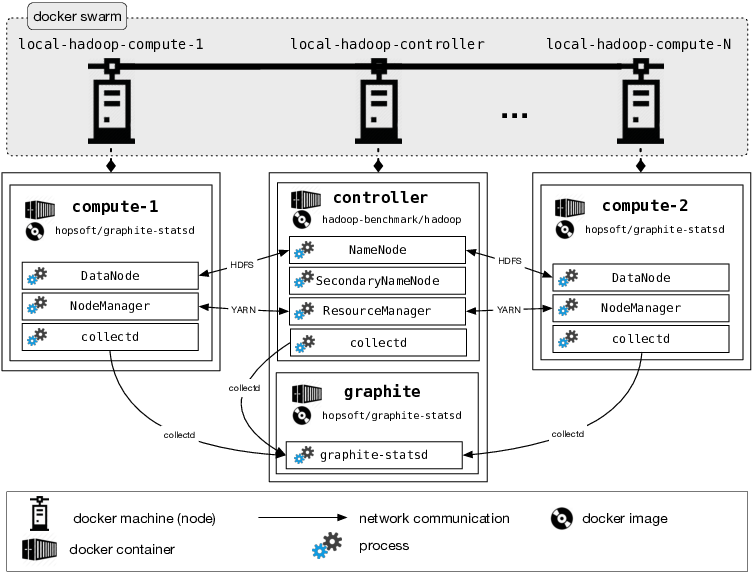
\includegraphics{./resources/hadoopBenchmarkArch.png}
    \caption[High"=Level"=Architektur von Hadoop"=Benchmark]
    {High"=Level"=Architektur von Hadoop"=Benchmark (entnommen aus \cite{abb:hadoopBenchmarkArch})}
    \label{fig:hadoopBenchmarkArchitecture}
\end{figure}

Mit \emph{Graphite}\footnote{\url{https://graphiteapp.org/}} ist zudem ein Monitoring"=Tool enthalten, mit dem die Systemwerte, wie CPU- oder Speicher"=Auslastung des Clusters, überwacht werden können.
Jeder Hadoop"=Container enthält dazu das Tool \emph{collectd}\footnote{\url{https://collectd.org/}}, was das Monitoring des Containers auf Systemebene übernimmt und die Daten an Graphite übermittelt.

Da mithilfe der Plattform auch unterschiedliche Hadoop"=Konfigurationen ausgeführt werden können, ist die Plattform in mehrere Szenarien unterteilt.
Jedes Szenario stellt eine vollständig anpassbare Hadoop"=Konfiguration dar.
Ein Szenario enthält dafür eine \emph{Dockerfile}, aus der die Docker"=Images und -Container erstellt werden, weitere für Hadoop benötigte Daten und Einstellungen sowie dazugehörige, generelle Einstellungen des Szenarios.
Die Plattform enthält bereits mehrere Szenarien, \uA Hadoop in einer Standardinstallation und ein darauf basierendes Szenario mit der Selfbalancing"=Komponente.
Aufgrund eines der Kernkonzepte von Docker, wonach Docker"=Images auf einem passenden, bereits vorhandenen Image aufbauen können bzw. sollten \cite{DockerdevBestPractice}, können neue Szenarien, basierend auf bereits vorhandenen, entwickelt werden.

Zum Starten des Clusters ist zudem ein Script enthalten, welches, basierend auf dem zu nutzenden Szenario das Cluster, in der entsprechenden Konfiguration startet.

In der Plattform Hadoop"=Benchmark sind auch bereits folgende Benchmarks integriert:

\begin{itemize}
    \item Hadoop"=Mapreduce"=Examples
    \item Intel HiBench\footnote{\url{https://github.com/intel-hadoop/HiBench/}}
    \item \gls{SWIM} \footnote{\url{https://github.com/SWIMProjectUCB/SWIM/}}
\end{itemize}

Die Benchmarks werden ebenfalls mithilfe der in der Plattform enthaltenen Scripte gestartet.
Hierbei besitzt jede Benchmark ein eigenes Start"=Script, das die Benchmark in einem Docker"=Container startet und die entsprechende Anwendung so dem Cluster zur Ausführung übergibt.
Die Ausführung sowie das Beenden einer Anwendung mithilfe der Scripte ist in \cref{app:hadoopCmds} beispielhaft aufgezeigt.

Genauere Informationen zu den in der Plattform enthaltenen Benchmarks sind in \cref{sec:appOverview} erläutert.
